
\section*{HS 1. feladat: Kazánfalon áthaladó hőmennyiség}
\addcontentsline{toc}{section}{HS 1. feladat}


\begin{tabular}{ | p{2cm} | p{14cm} | } 
	\hline
	Név & Kovács Bence \\ 
	\hline
	Szak &  Mechatronikai mérnöki alapszak\\
	\hline
	Félév & 2019/2020 II. (tavaszi) félév \\ 
	\hline
\end{tabular}
\vspace{0.5cm}

Határozza meg azt a hőmennyiséget, amely a kazánfal $A_1$ felületén óránként átadódik, ha a fal vastagsága $\delta_1$, anyagának hővezetési tényezője $\lambda_1$ és a fal belső oldalát $\delta_2$ vastag kazánkő réteg borítja, aminek a hővezetési tényezője $\lambda_2$. A kazán falának füstgázoldali hőmérséklete $T_1$, vízoldali hőmérséklete $T_2$. Számítsa ki a kazán falának közepes hőmérsékletét és rajzolja fel a hőmérséklet-hely függvényt léptékhelyesen!
    \vspace{1mm}

\subsubsection*{Adatok:}
\vspace{1mm}

    ($\lambda_1 = \SI{45}{\watt\per\meter\K}$ ;
    $\lambda_2 = \SI{1.5}{\watt\per\meter\K}$ ;
    $A_1 = \SI{1}{\meter^2}$ ; 
    $\delta_1 = \SI{20}{\milli\meter}$ ; 
    $\delta_2 = \SI{2}{\milli\meter}$ ; 
    $T_1 = \SI{260}{\celsius}$ ; 
    $ T_2 = \SI{195}{\celsius}$ )
    \vspace{3mm}

\hline
\subsubsection*{Megoldás:}

Először felírjuk a hőáramsűrűségre vonatkozó egyenletet:

\begin{equation*}
	 \dot{q} = \frac{\lambda_1}{\delta_1} (T_1 - T_2)
\end{equation}

Majd ezt külön kiszámoljuk a kazánfal 2 oldalára, beleértve a $\SI{2}{\milli\meter}$ vastag kazánkő réteget is. Mivel a kazánkő réteg és a kazánfal érintkezési felületénél nem ismerjük a hőmérsékletet, ezt paraméteresen $T_3$-mal számoljuk.:

\begin{equation}
	 \dot{q}_1 = \frac{\SI{45}{\watt\per\meter\K}}{\SI{0.02}{\meter}} (\SI{533.15}{\kelvin} - T_3)
\end{equation}


\begin{equation}
	 \dot{q}_2 = \frac{\SI{1.5}{\watt\per\meter\K}}{\SI{0.002}{\meter}} (T_3 - \SI{468.15}{\kelvin})
\end{equation}


\begin{equation}     
     \dot{q}_1 = \SI{2250}{\watt\per\kelvin} \cdot (\SI{533.15}{\kelvin} - T_3)
\end{equation}


 \begin{equation}   
    \dot{q}_2 = \SI{750}{\watt\per\K} \cdot (T_3 -  \SI{468.15}{\kelvin})
\end{equation}

    Mivel az energimegmaradás és az állandósult állapot miatt a két réteg hőáramsűrűsége egyenlő, így az alábbi egyenletet kapjuk:
\begin{equation}    
    \SI{2250}{\watt\per\kelvin} \cdot (\SI{533.15}{\kelvin}-T_3) = \SI{750}{\watt\per\K}(T_3-\SI{468}{\kelvin})
\end{equation}


\begin{equation}
    \SI{1599,45}{\kelvin}-3 \cdot T_3 = T_3-\SI{468.15}{\kelvin}
\end{equation}
        
Ebből $T_3$-at kifejezve, megkapjuk az érintkezési felület hőmérsékletét:

\begin{equation}
    T_3 = \frac{\SI{2067.6}{\kelvin}}{4} = \SI{516,9}{\kelvin} = \SI{243,73}{\celsius}
\end{equation}
    
    Visszahelyettesítve az eredeti egyenletbe, megkapjuk a kazánfalon átadódó hőmérsékletet:
\begin{equation}
     \dot{q} = \SI{750}{\watt\per\K} \cdot (\SI{516,9}{\kelvin} - \SI{468.15}{\kelvin}) = \SI{36562,5}{\watt\per\meter\squared} 
\end{equation}
    
A közepes hőmérséklethez az alábbi egyenletet használjuk fel:
\begin{equation}
     T_K = T_1- \frac{T_1 - T_2}{\delta_1} \cdot x
\end{equation}
\vspace{0.5cm}

x a kazánfal vastagság fele.

Mivel a változók ismertek, behelyettesítve az egyenletbe megkapjuk a kívánt értéket.
\begin{equation}
     T_K = \SI{533.15}{\kelvin} - \frac{\SI{533.15}{\kelvin} - \SI{516.9}{\kelvin}}{\SI{0.02}{\meter}} \cdot 0.01 =  \SI{525.025}{\kelvin} =  \SI{251.87}{\celsius}
\end{equation}
        
\vspace{0.5cm} 
\subsubsection*{A Feladat kiszámítása után ábrázoljuk a hőmérséklet-hely függvényt:}
\vspace{0.5cm} 
        
    \begin{figure}[h]
	\centering

		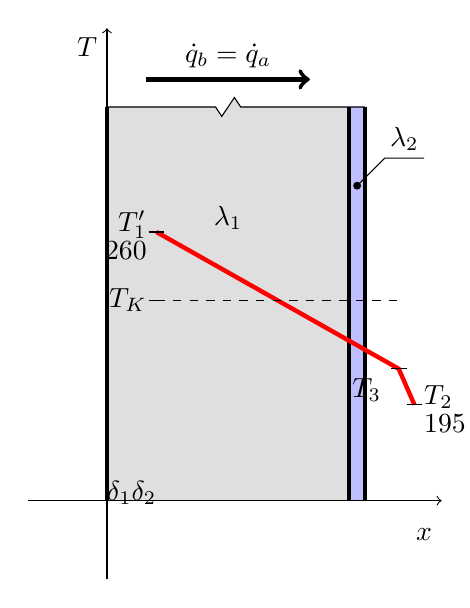
\begin{tikzpicture}
			\pgfmathsetmacro{\d}{20/6.5}
			\pgfmathsetmacro{\v}{1.2/6}
			\pgfmathsetmacro{\L}{5}
			\pgfmathsetmacro{\TA}{260/160*2.1}
			\pgfmathsetmacro{\TB}{243.73/160*1.1}
			\pgfmathsetmacro{\TC}{195/160}
			\pgfmathsetmacro{\TK}{(\TA+\TB)/2}
			
			% Fal
			\fill[gray,opacity=0.25] (0,0) -- (0,\L) -- ({\d/2-0.16},\L) -- ({\d/2-0.08}, {\L-0.12}) -- ({\d/2+0.08}, {\L +0.12}) -- ({\d/2+0.16}, \L) -- (\d, \L) -- (\d, 0);
			\fill[blue,opacity=0.25] (\d, \L) -- (\d, 0) -- (\d+\v, 0) -- (\d+\v, \L);
			\draw[] (0,\L) -- ({\d/2-0.16},\L) -- ({\d/2-0.08}, {\L-0.12}) -- ({\d/2+0.08}, {\L+0.12}) -- ({\d/2+0.16}, \L) -- (\d, \L) -- (\d+\v, \L);
			\draw[ultra thick] (0,0) -- (0,\L);
			\draw[ultra thick] (\d, 0) -- (\d, \L);
			\draw[ultra thick] (\d+\v, 0) -- (\d+\v, \L);
			
			% Tengelyek
			\draw[->] (0,-1) -- (0,\L+1) node[anchor=north east]{$T$};
			\draw[->] (-1,0) -- (4.25,0) node[anchor=base east, shift={(0,-0.5)}]{$x$};
			
			% Hőáram és hőáramsűrűség
			\draw[->, ultra thick] (0.5,{\L+0.35}) -- ({\d/2},{\L+0.35}) node[anchor=south]{$\dot{q}_b = \dot{q}_a$} -- ({\d - 0.5},{\L+0.35});
			
			% A hővezetési tényező
			\node[anchor=base] at ({\d/2},{\L-1.5}) {$\lambda_1$};
			\node[anchor=base] at ({\d+\v+0.5},{\L-0.5}) {$\lambda_2$};
			\draw ({\d+\v+0.75},{\L-0.65}) -- ({\d+\v+0.25},{\L-0.65}) -- ({\d+\v/2},{\L-1});
			\fill[] ({\d+\v/2},{\L-1}) circle[radius=0.05];
			
			% A falvastagságok
			\pgflength[xa=0, ya=0, xb=\d, yb=0, alim=0]{$\delta_1$};
			\pgflength[xa=\d, ya=0, xb=\d+\v, yb=0, alim=0, a=0, belül=2]{$\delta_2$};
			
			% T(x)
			\draw[red, ultra thick] (0,\TA) -- (\d,\TB) -- (\d+\v,\TC);
			
			% Falhőmérsékletek
			\draw (-0.1,\TA) -- (0.1,\TA);
			\node[anchor=base east] at (0,\TA) {$T_1'$};
			
			\draw (-0.1+\d,\TB) -- (0.1+\d,\TB);
			\node[anchor=north east] at (\d-0.1,\TB) {$T_3$};
			
			\node[anchor=north east] at (0,\TA) {$\SI{260}{\celsius}$};
			
			\draw (-0.1+\d+\v,\TC) -- (0.1+\d+\v,\TC);
			\node[anchor=base west] at (\d+\v,\TC) {$T_2$};
			\node[anchor=north west] at (\d+\v,\TC) {$\SI{195}{\celsius}$};
			
			% A közepes hőmérséklet
			\draw[dashed] (0,\TK) -- (\d,\TK);
			\draw (-0.1,\TK) -- (0.1,\TK);
			\node[anchor=east] at (0,\TK) {$T_K$};
			
		\end{tikzpicture}
		\caption{Hőmérséklet-hely függvény}

\end{figure}

\pagebreak
